\chapter{Testes e Resultados}\label{cap:resultados}

\section{Protocolos de teste}
\label{sec:res-protocolos}

Em junho de 2026, caracterizaram-se o IMU, com um participante e sem o
colar final, e três FSR402, com cargas sobre balança. Avaliaram-se posturas,
recolocações do IMU, carga/descarga e acomodação dos FSRs.

Em 21/10/2026, nove sessões com oito participantes registraram o sistema
com motor mudo. As posturas instruídas foram: (1) ereto, (2) curvado à
frente, (3) cabeça à frente com tronco apoiado, (4) escorregado,
(5--6) inclinado à esquerda/direita, (7) reclinado e (8--9) perna
esquerda sobre direita/direita sobre esquerda. Espera-se alerta em 2--6.
Mantiveram-se as posturas por cerca de 15\,s; aproveitaram-se 123 segmentos
e 50{,}74\,min com calibração válida, sem transições e os 2\,s iniciais.
Os rótulos são instruções do operador, sem medida anatômica independente.

Compararam-se as regras por reprodução temporal (\textit{replay}). No LOSO
(\textit{leave-one-subject-out}), ajustam-se os parâmetros com sete sujeitos
e avalia-se o omitido; as sessões de André ficam juntas. A pontuação
balanceada é a média entre tempo alertado nos segmentos prejudiciais e
não alertado nos aceitáveis, incluindo pernas cruzadas, com igual peso por
segmento em cada grupo. Em 22/10, duas sessões em hardware usaram motor
ativo, com participante conhecido e sujeito novo.

\section{Caracterização em bancada}
\label{sec:res-bancada}

Nas quatro remontagens de bancada, a referência ereta variou cerca de
8\degree{} em \textit{pitch} e 21{,}6\degree{} em \textit{roll},
sustentando a calibração após vestir o colar. Nos FSRs, a histerese média
absoluta foi próxima de 52\,\% até 400\,g e 6\,\% a partir de 1\,kg.
Sob 1\,kg constante, a resistência caiu 7{,}4\,\% e 11{,}5\,\% em dois
sensores, em cerca de 11 e 12 minutos. A não linearidade, a histerese e o
\textit{creep} justificam medidas relativas à linha de base individual.

\section{Detecção nas capturas integradas}
\label{sec:res-deteccao}

A Figura~\ref{fig:res-dispersao} mostra a dispersão entre pessoas e
colocações no espaço absoluto, reduzida no ereto pela calibração.
Ainda assim, escorregado e reclinado se sobrepõem: suas médias
$(\Delta p,\Delta r)$ são $(-1{,}1;10{,}7)\degree{}$ e
$(-1{,}0;13{,}5)\degree{}$. A orientação isolada não informa o apoio do
quadril, o que motiva os FSRs.

\begin{figure}[H]
  \centering
  \caption{Dispersão angular nas capturas integradas: amostras estáveis
  e média $\pm1\sigma$ por postura, reunindo os oito participantes.}
  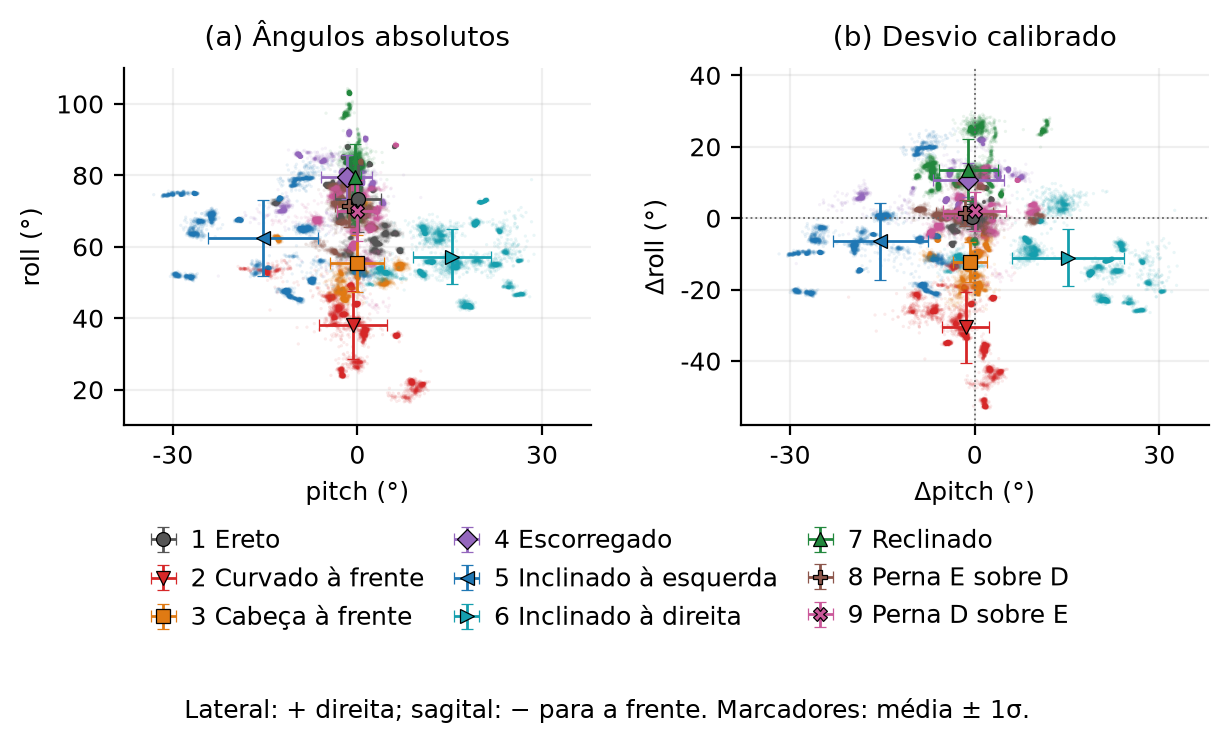
\includegraphics[width=\linewidth]{res_dispersao_posturas.png}
  \fonte[Fonte]{Elaborado pelos autores (2026)}
  \label{fig:res-dispersao}
\end{figure}

A Tabela~\ref{tab:res-comparacao} compara o mesmo recorte. A fusão final
foi ajustada com todos os dados; o LOSO avalia a transferência ao sujeito
omitido. A regra só-IMU não foi ajustada a essas capturas. Considera-se
detectado o segmento com ao menos um alerta, mesmo iniciado antes do
rótulo; por isso, informa-se também o tempo alertado.

\begin{table}[H]
  \centering
  \caption{Detecção por replay nas capturas de 21/10/2026.}
  \begingroup\SingleSpacing
  \small
  \begin{tabularx}{\linewidth}{@{}Xccc@{}}
    \toprule
    Indicador & Só-IMU & Fusão final & Fusão LOSO \\
    \midrule
    Segmentos prejudiciais detectados & 55/62 & 58/62 & 58/62 \\
    Tempo prejudicial com alerta (\%) & 84 & 93 & 92 \\
    Tempo ereto/reclinado com alerta (\%) & 29 & 2 & 3 \\
    Tempo de pernas cruzadas com alerta (\%) & 10 & 11 & 28 \\
    Pontuação balanceada por segmento & 0{,}834 & 0{,}935 & 0{,}901 \\
    \bottomrule
  \end{tabularx}
  \fonte[Fonte]{Elaborado pelos autores (2026)}
  \label{tab:res-comparacao}
  \endgroup
\end{table}

Na Figura~\ref{fig:res-alerta-sujeitos}, curvar à frente, escorregar e
inclinar à esquerda alertaram durante todo o recorte com a fusão final.
Cabeça à frente falhou em três de sete participantes: o movimento
localizado pouco alterou o IMU e preservou o contato. À direita de
Vinicius, desvio próximo ao limiar e carga oposta à esperada limitaram
o alerta a 38\,\% do tempo.

\begin{figure}[H]
  \centering
  \caption{Tempo com alerta por participante e postura: fusão final.}
  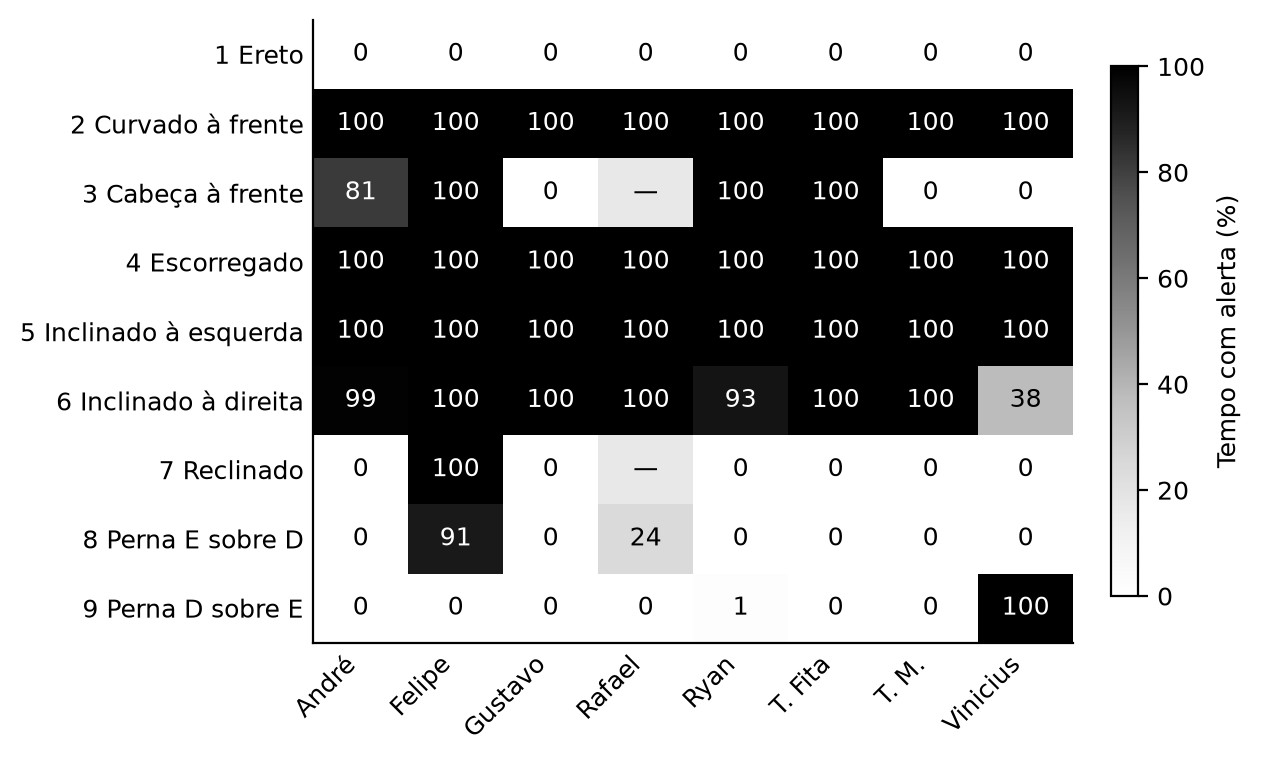
\includegraphics[width=\linewidth]{res_alerta_sujeitos.png}
  \fonte[Fonte]{Elaborado pelos autores (2026)}
  \label{fig:res-alerta-sujeitos}
  \begingroup\SingleSpacing
  {\footnotesize Espera-se alerta nas linhas 2--6 e ausência nas demais;
  células escuras indicam mais alerta, não necessariamente acerto. Traço:
  postura não registrada. E/D: esquerda/direita; T. Fita/T. M.: Thiago
  Fita/Thiago M.}
  \endgroup
\end{figure}

Em Felipe, desvio lateral próximo de 10\degree{} sem alteração no
assento foi compatível com deslocamento do colar e gerou falsos alarmes.
Vinicius escorregou ao cruzar as pernas: um alerta justificável foi contado
como falso pelo rótulo. Na ablação cumulativa, o maior ganho veio do
tratamento da reclinação apoiada; a confirmação lateral também acrescentou
falsos alarmes com pernas cruzadas.

\section{Validação em hardware e mostra}
\label{sec:res-hardware}

Na rodada guiada de André, participante do desenvolvimento, o alerta
nas placas ocupou 100\,\% do tempo estabilizado de 2--6 e 0\,\% das
demais posturas. Perceberam-se a vibração e sua interrupção ao retornar ao
ereto, verificando sensores, decisão e atuação.

Lucas, sujeito novo, realizou roteiro parcial: curvar à frente e escorregar
alertaram em 100\,\% do tempo estabilizado; inclinar à direita não
alertou. À esquerda, o alerta ocupou 9{,}2\,\%: a vibração perturbou o
IMU em cerca de $\pm10\degree{}$, interrompendo o alerta e reiniciando
os 3\,s. A correção reteve a última orientação sem motor durante a
vibração e elevou o alerta a 100\,\% no replay, sem nova sessão controlada
em hardware para confirmá-la.

Na mostra Eureka, em novembro, mais de 150 visitantes de biotipos
variados usaram o sistema com calibração individual e retorno vibratório;
a postura prejudicial foi detectada em praticamente todos os casos
observados, e os erros limitaram-se ao nome exibido para movimentos
combinados. Sem capturas rotuladas, essa evidência é qualitativa e não
integra os percentuais. O colar operou com uma célula de 600\,mAh durante
os dois dias (cerca de 20\,h) sem esgotá-la, o que indica corrente média
de no máximo cerca de 30\,mA; por extrapolação proporcional à capacidade
nominal, a célula de 1800\,mAh daria da ordem de 60\,h, valor não medido.

\section{Discussão}
\label{sec:res-discussao}

Com a fusão final, o alerta no reclinado caiu de 78\,\% para 5\,\%
do tempo; no escorregado, subiu de 72\,\% para 100\,\%. Em cerca de
176\,s de cadeira vazia, caiu de 71\,s para zero. O ganho decorre do
apoio e da presença medidos no assento; não se demonstrou contribuição
equivalente dos oito FSRs. Detectar o desvio é o objetivo; nomear posturas
mistas é complementar.

As capturas instruídas com oito participantes e um novo na validação
demonstram viabilidade, sem ensaio prolongado ou inferência populacional.
Persistem falhas com cabeça à frente, deslocamento do colar e posturas
mistas. Não alertar por pernas cruzadas é opção de escopo, sem conclusão
clínica. Não se mediram corrente e latência em bancada nem efeitos
duradouros sobre hábitos ou distúrbios musculoesqueléticos.
